\begin{figure}
	\centering
	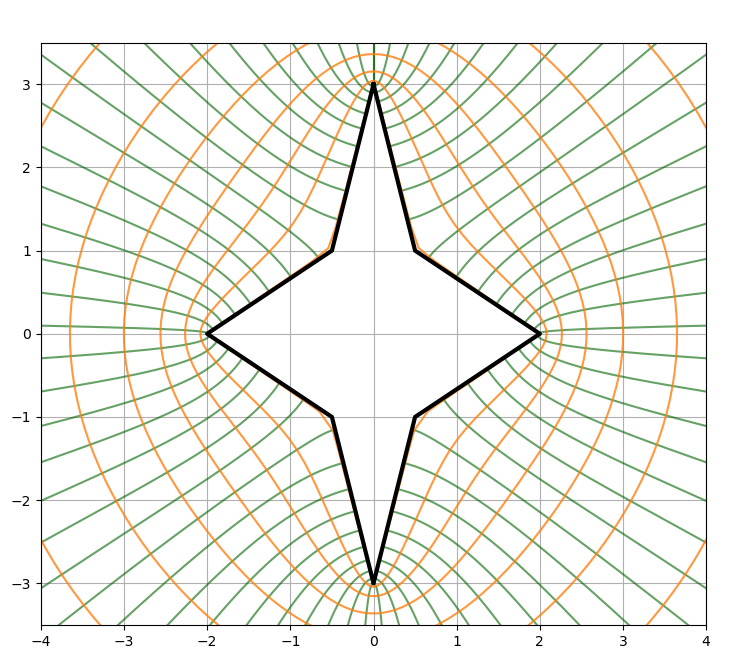
\includegraphics[width=\textwidth]{papers/elektro/grafik/SC_trafo_star.png}
	\caption{Sternförmige Kontur mit unterschiedlich grossen Innenwinkeln.
	An den spitzen Bereichen liegen die elektrischen Feldlinien dichter beieinander, was auf eine grössere elektrische Feldstärke hinweist.}
	\label{elektro:figure:SC_star_trafo}
\end{figure}
